\documentclass{beamer}
\usetheme{default}
\usepackage{array}
\usepackage{graphicx}
\usepackage{multimedia}
\usepackage{media9}
\usepackage{adjustbox}

\setbeamertemplate{footline}[text line]{%
	\parbox{\linewidth}{\vspace*{-8pt}Repository: https://github.com/domenicus/VR-Mapping}}
\setbeamertemplate{navigation symbols}{}

\defbeamertemplate*{title page}{customized}[1][]
{
	\begin{columns}
		\begin{column}{.5\textwidth}
			\usebeamerfont{title}\inserttitle\par
			\usebeamerfont{subtitle}\usebeamercolor[fg]{subtitle}\insertsubtitle\par
			\bigskip
			\usebeamerfont{author}\insertauthor\par
			\usebeamerfont{institute}\insertinstitute\par
			\usebeamerfont{date}\insertdate\par
		\end{column}
		\begin{column}{.5\textwidth}
			\ifx\useflashembed\undefined
					\immediate\write18{%
						pdflatex --jobname=\jobname-flash "\gdef\string\useflashembed{0}\space\string\input\space\jobname"%
					}
				\movie[label=show3,width=1.0\textwidth,poster,autostart,loop]%
				{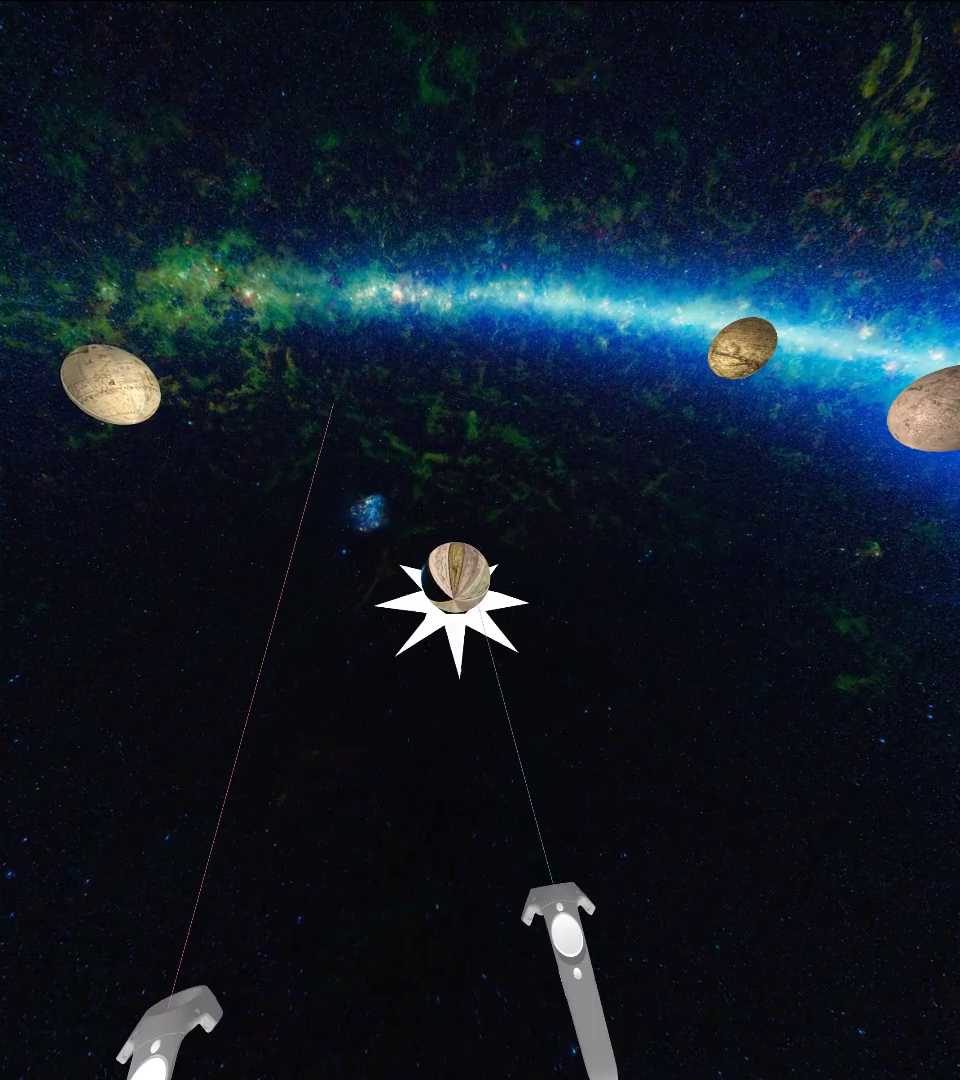
\includegraphics[width=1.0\textwidth]{intro-video.png}}{intro-video.mp4}
			\else%Try bad flash player first??
				\includemedia[
				  width=\textwidth,
				  height=0.7\textheight,
				  activate=pageopen,
				  addresource=intro-video.mp4,
				  flashvars={
				    %important: same path as in `addresource'
				    source=intro-video.mp4 %
				    &scaleMode=stretch %
				    &autoPlay=true %
				    &autoRewind=true %
				    &loop=true %
				  }
				]{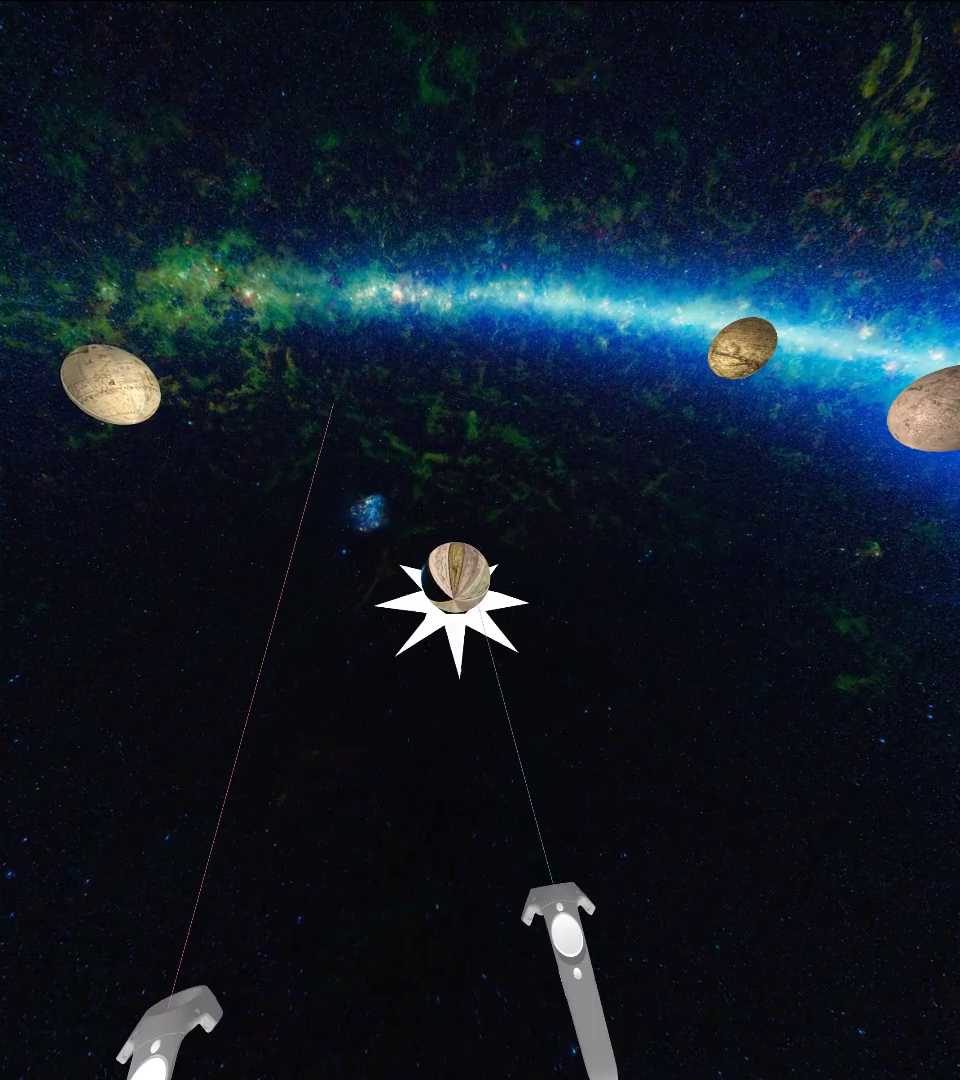
\includegraphics[width=1.0\textwidth]{intro-video.png}}{VPlayer.swf}
			\fi
		\end{column}
	\end{columns}
}

\title{On Exactitude In Science: Semiotics Of Representations}
\subtitle{Early Modern Maps \& [Virtual] Reality}
\author{Prof. Domingo Ledezma, Prof. Evelyn Staudinger, and Noah Cowie '21}
\date{\today}


\begin{document}

\maketitle

\begin{frame}{On Exactitude in Science, by Jorges Luis Borges}
	... In that Empire, the Art of Cartography reached such Perfection that the map of a single
	Province occupied a whole City, and the map of the Empire a whole Province. In the course
	of time, these Disproportionate Maps were found wanting, and the Colleges of Cartographers
	elevated a Map of the Empire that was of the same scale as the Empire and coincided with it
	point for point. Less Fond of the Study of Cartography, Subsequent Generations understood
	that such an expanded Map was Useless, and not without Irreverence they abandoned it to the
	Inclemencies of the Sun and of Winters. In the deserts of the West, tattered Ruins of the Map
	still abide, inhabited by Animals and Beggars; in the whole Country there is no other relic of
	the Disciplines of Geography.\par

	\hfill Su\'arez Miranda, Travels of Prudent Men, Book Four, Ch. XLV, L\'erida, 1658\par
\end{frame}

\begin{frame}{Del Rigor en la Ciencia de Jorge Luis Borges}
	... En aquel Imperio, el Arte de la Cartografía logr\'o tal Perfecci\'on que el mapa de una sola
	Provincia ocupaba toda una Ciudad, y el mapa del Imperio, toda una Provincia. Con el
	tiempo, estos Mapas Desmesurados no satisficieron y los Colegios de Cart\'ografos levantaron
	un Mapa del Imperio, que ten\'ia el tama\~no del Imperio y coincid\'ia puntualmente con \'el.
	Menos Adictas al Estudio de la Cartografía, las Generaciones Siguientes entendieron que ese
	dilatado Mapa era In\'util y no sin Impiedad lo entregaron a las Inclemencias del Sol y los
	Inviernos. En los desiertos del Oeste perduran despedazadas Ruinas del Mapa, habitadas por
	Animales y por Mendigos; en todo el Pa\'is no hay otra reliquia de las Disc\'iplinas Geogr\'aficas.\par

	\hfill Su\'arez Miranda, Viajes de Varones Prudentes, Libro Cuarto, Cap. XLV, L\'erida, 1658\par

\end{frame}
\begin{frame}{Cartography}
	\begin{enumerate}
		\item Maps are everywhere
		\item Maps are complex graphical, representational, and narrative objects

		\item Medieval  mapping technologies concerned themselves as much with symbolic relationships among peoples, places, and the unknown (including the spiritual)

		\item As mediators between an inner mental world and an outer physical world, maps are fundamental tools helping the human mind make sense of its universe at various scales.

		\item To represent is to signify ... to create meanings:
		\item In relation to semiology is that maps form a system of signification (semiotics)
	\end{enumerate}
\end{frame}
\begin{frame}
	``Semiology ... aims to take in any system of signs, whatever their substance and limits; images, gestures, musical sounds, objects, and the complex association of all these, which form the content of ritual, convention or public entertainment: these constitute, if not languages, at least systems of signification.''\par
	\hfill Roland Barthes, Elements of Semiology\par
\end{frame}

\begin{frame}{About Reality}
	\begin{enumerate}
		\item Esse est percipi: ``to be is to be perceived''
		\item According to this argument 18th-century Anglo-Irish empiricist George Berkeley, all the qualities attributed to objects are sense qualities.

		\item Maps as representations, an objectification of space, produce and project a reality that in western tradition has been accepted as ``reality'' … remember the arrow in a map telling: ``you are here''

		\item Virtual reality as we currently understand it, it’s an immersion experience in a 3D computer generated environment. 
	\end{enumerate}

	``We accept reality so readily - perhaps because we sense that nothing is real.''\par
	\hfill Jorge Luis Borges \par
\end{frame}

\begin{frame}{Why is a map different in a VR Space}
	\textit{Why VR is better than reality for observing a map, playing with a map?}
	\begin{enumerate}
		\item Iteractivity: zooming, voice-over, text, animation
		\item Ease of focus: the eye is focused on a single object: the
			vision is captured by a giant image of representation of space
		\item Map of maps: the ability to browse a huge catalog of map in a single
			space, and to curate that huge map
		\item Inhabiting a map; recreating a map as 3D space. Gaming maps.
	\end{enumerate}
\end{frame}

\begin{frame}{The paradox of Exactitude in Science.}
	\begin{enumerate}
		\item The map of scale 1:1 is being constructed by the internet, 
			actually AR: The Mirror World.
		\item VR and the Inner mirror: The Inner map of knowledge
		\item We propose to go inside the object of knowledge: in this case Early Modern Maps but it could be any knowledge
		\item The Aleph is an sphere in which all places of the universe are located is the universe.
		\item We place an Aleph on a compass:  that sphere is actually an entrance to a constellation of planets inhabited by knowledge
	\end{enumerate}
\end{frame}
\begin{frame}
	``Truth cannot penetrate a closed mind. If all places in the universe are in the Aleph, then all stars, all lamps, all sources of light are in it, too.''\par

	``Of course, if you don’t see it, your incapacity will not invalidate what I have experienced.''
\end{frame}



\begin{frame}{Technical Aspects}
	\begin{enumerate}
		\item Software toolchain
		\item How to make reality convincing
		\item Example: compass
		\item Example: voices
	\end{enumerate}
\end{frame}
\begin{frame}{Software toolchain}
	\begin{enumerate}
		\item We deliver all content through the browser. All of our code is
			JavaScript and HTML. 
		\item We do not have a serverside component; any HTTP
			server will do (e.g. Apache, Nginx).\\
		\item To access VR we depend on the WebVR browser API, the
			Gamepad API, and the A-Frame JavaScript library.
		\item Firefox controls the headset on our behalf through SteamVR.
	\end{enumerate}
\end{frame}
\begin{frame}{Why A-Frame}
	\begin{columns}[t]
		\begin{column}{.3\textwidth}
			\adjincludegraphics[width=.8\linewidth,valign=t]{aframe}
		\end{column}
		\begin{column}{.7\textwidth}
	When we set out, we wanted to ensure we weren't tied to a single headset
	or a single computer. The easiest way to achieve this is to use a
	headset-agnostic, OS-agnostic framework like A-Frame.\\
	A-Frame is completely open source, meaning that we can make our own
	modified copies and keep and distribute them without issue. This avoids
	relying on a commercial software licencing agreement for future availability.
		\end{column}
	\end{columns}
\end{frame}
\begin{frame}{How to make reality convincing}
	We started with very basic environments, like rooms with flat maps on
	the wall. We learned a variety of important lessons:
	\begin{enumerate}
		\item Sharp transitions are scary, slow transitions are
			nauseating.
		\item Turning around is annoying.
		\item Boring space is bad space.
	\end{enumerate}
	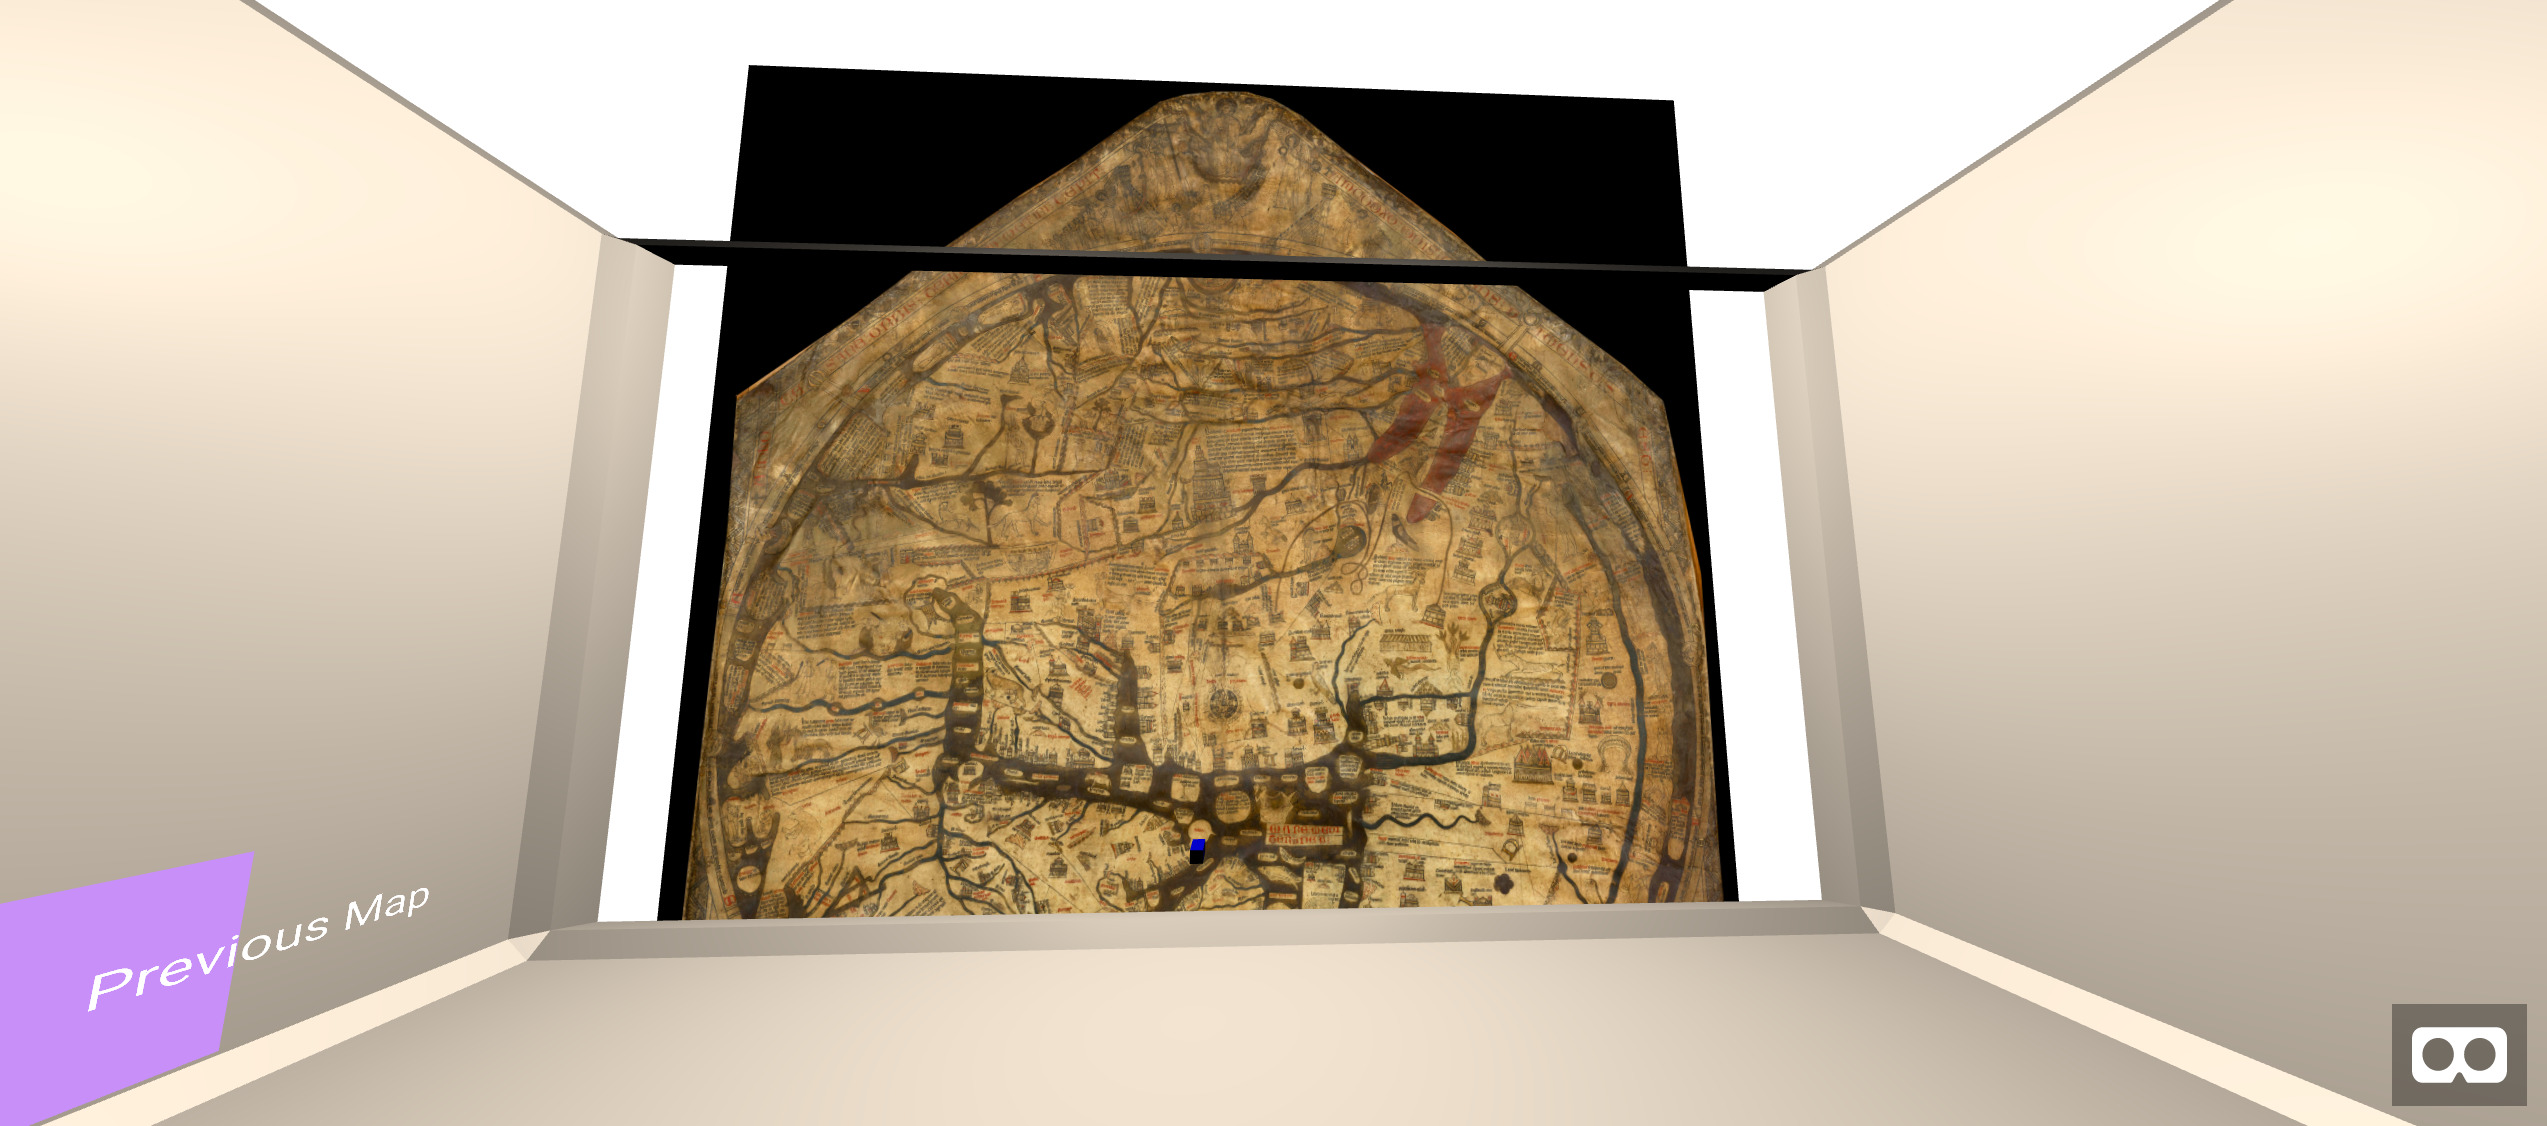
\includegraphics[width=\textwidth]{early}
\end{frame}
\begin{frame}{Compass}
	\begin{columns}[t]
		\begin{column}{.3\textwidth}
			\adjincludegraphics[width=.8\linewidth,valign=t]{portal}
			\adjincludegraphics[width=.8\linewidth,valign=t]{portal2}
		\end{column}
		\begin{column}{.7\textwidth}
	\begin{enumerate}
		\item At first, we just started people in front of a map.
			This was not exciting.
		\item So, we added an introductory space, with a 'portal' to get in.
			We made our 'portal' by putting an image on the 'inside' of a globe,
			and making the walls transparent from the outside.
		\item We ultimately transformed the introductory space to the literal vision
			of space we now have, but the portal had captured out attention as
			the 'Aleph' from Borges.
		\item We kept the portal, since it was a good (and philosophically satisfying)
			transition.
	\end{enumerate}
		\end{column}
	\end{columns}
\end{frame}
\begin{frame}{Compass}
	\begin{columns}[t]
		\begin{column}{.3\textwidth}
			\adjincludegraphics[width=.8\linewidth,valign=t]{compass}
		\end{column}
		\begin{column}{.7\textwidth}
	\begin{enumerate}
		\item To really have an Aleph, we needed to be able to access
			\textbf{all} the maps, not just one.
		\item We put all the maps in one little portal, and let the user select which
			one they want. This was also very convenient!
		\item We decided to use a motif from one of the maps we studied, a compass.
		\item We made a 3D model and attached it to the portal, making it feel more physical.
	\end{enumerate}
		\end{column}
	\end{columns}
\end{frame}
\begin{frame}{Voices}
	\begin{enumerate}
		\item We first experimented with having a box of information on one side of the screen.
		\item Reading text in VR is both boring and occasionally difficult.
		\item So, we decided to have voice annotations. 
		\item We created a flat, non-VR tool to
			graphically map audio files onto the map.
		\item We used to play audio whenever the user looked at the right area, but it was
			annoying.
		\item We play the audio back when the user zooms in -- giving them context only
			when they ask for it.
	\end{enumerate}
	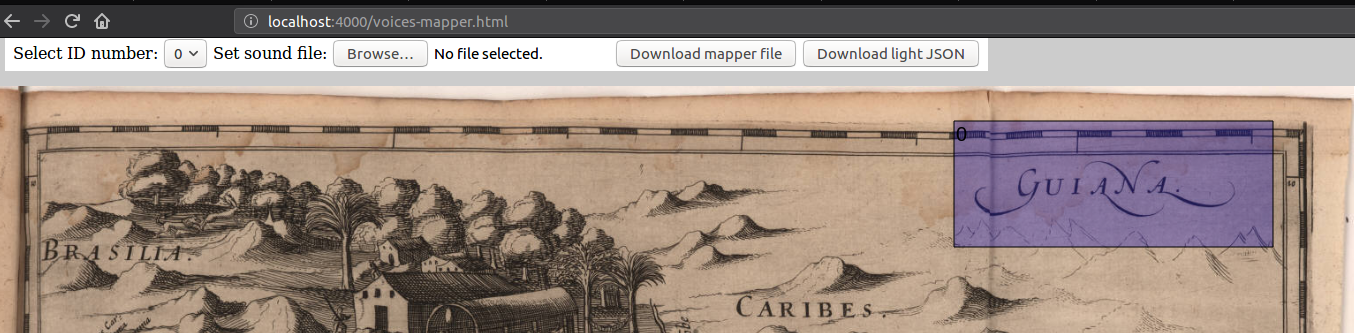
\includegraphics[width=\linewidth]{voices-mapper}
\end{frame}

\end{document}
